    \chapter{Solution of Nonlinear Equations}
    We would like to find the roots of equations of the form $f(x) = 0$
    We will focus on the one-dimensional case (in which $f:[a, b] \rightarrow \mathbb{R}$)
    In several dimensions one is often interested in solving several simultaneous equations.
    This can be hard.
    We will look at several iterative methods: Bisection, Regula Falsi, Secant Method, Newton's Method
    Other methods include Fixed Point Iteration and various hybrid methods (see NRiC). 
    Later we will discuss the special cases in which $f$ is a polynomial or a linear function in higher dimensions. 
    \subsection*{Applications}
    \begin{itemize}
        \item Intersection / collision detection
        \item Optimization (we'll see the connection later)
    \end{itemize}
    
    \section{Bisection}
    \textbf{Idea:}
        \begin{description}
            \item Find two points $a_0, b_0$ such that $f(a_0) * f(b_0)$ have opposite signs. 
            If $f$ is well-behaved, then it will have a root in between $a_0 * b_0$. 
            Now, halve the interval $[a_0, b_0]$ while still bracketing the root, and repeat
        \end{description}
    
    \textbf{Formally:}
    Start with $f(a_0)f(b_0) \leq 0$
    For $n = 0, 1, 2, ...$ until satisfied do:
    $c = \frac{1}{2}(a_n + b_n)$
    If $f(a_n)f(c_n) \leq 0$, then set $a_{n+1} = a_n; b_{n+1} = c$
    else set $a_{n+1} = c; b_{n+1} = b_n$
    
    
    \noindent \underline{Comments}
    \begin{itemize}
        \item The first part of the idea is critical to many root-finding techniques namely to find an interval that brackets a root of $f$. 
        This can be difficult.
        \item Bisection can be slow, but it is simple and robust. 
        It is therefore sometimes used as a "fail safe" backup for more complicated algorithms. 
    \end{itemize}

    \begin{figure}
      \centering
      \begin{subfigure}[b]{0.3\textwidth}
        \resizebox{\textwidth}{!}{
          \begin{tikzpicture}
\begin{axis}[
axis y line=center,
axis x line=middle,
scale only axis,
axis equal,
xmax=3,xmin=-3,
ymin=-4,ymax=4,
ticks=none,
width=5cm,
samples=100,
anchor=center,
]
\addplot[thick,domain=-5:0.9,mark=none]{-0.2*x/(1-x) -1};
\addplot[thick,domain=1.1:5,mark=none]{-x/(1-x) -1};
\addplot[thick,mark=none,dashed] coordinates {(1, -4) (1, 4)};
% \addplot[thick,mark=none,dashed] {-1};
\end{axis}
\end{tikzpicture}

        }
        \caption{Singularities}
      \end{subfigure}
      \begin{subfigure}[b]{0.3\textwidth}
        \resizebox{\textwidth}{!}{
          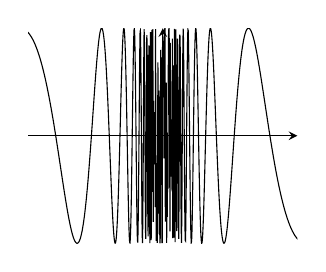
\begin{tikzpicture}
\begin{axis}[
axis y line=center,
axis x line=middle,
xmax=0.2,xmin=-0.2,
ymin=-1,ymax=1,
ticks=none,
width=5cm,
anchor=center,
]
\addplot [domain=-0.5:0.5,samples=2000] {sin(deg(1/x))};
\end{axis}
\end{tikzpicture}

        }
        \caption{Many Roots}
      \end{subfigure}
      \begin{subfigure}[b]{0.3\textwidth}
        \resizebox{\textwidth}{!}{
          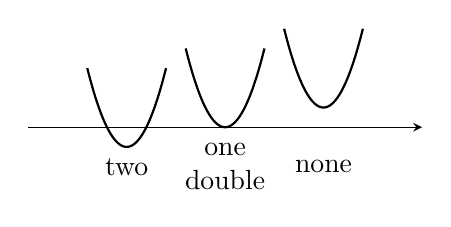
\begin{tikzpicture}
\begin{axis}[
axis y line=none,
axis x line=middle,
scale only axis,
axis equal,
ymin=-1,ymax=1,
xmin=-10,xmax=10,
ticks=none,
width=5cm,
samples=100,
anchor=center,
]
\addplot[thick,domain=-7:-3,mark=none]{(x+5)^2-1};
\addplot[thick,domain=-2:2,mark=none]{(x)^2};
\addplot[thick,domain=3:7,mark=none]{(x-5)^2+1};

\node[align=center] at (axis cs:0,-2) {one\\double};
\node at (axis cs:-5,-2) {two};
\node at (axis cs:5,-2) {none};
\end{axis}
\end{tikzpicture}

        }
        \caption{Double Roots}
      \end{subfigure}
      \label{fig:difficult-root-finding}
    \end{figure}

\newpage

    \subsubsection{Note:}
        \begin{description}
            \item The pseudo-code
            \item "If $f(a_n)f(c)n) \leq 0$..."
            \item Is just shorthand for
            \item "If $f(a_n)$ and $f(c_n)$ have opposite sign (or one is zero)..."
            \item Multiplication is probably not the best way to implement this test.
        \end{description}
    
    \begin{figure}
      \centering
      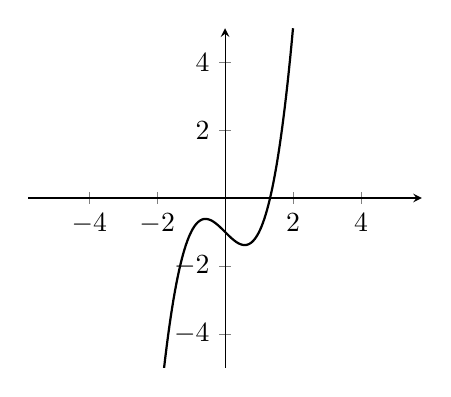
\begin{tikzpicture}
\begin{axis}[
axis y line=center,
axis x line=middle,
scale only axis,
axis equal,
xmax=2,xmin=-2,
ymin=-5,ymax=5,
width=5cm,
samples=100,
anchor=center,
]
\addplot[thick,domain=-2:2,mark=none]{x^3-x-1};
\end{axis}
\end{tikzpicture}

      \label{fig:bisection_example}
    \end{figure}
    \subsubsection{Note:}
        \begin{description}
            \item Since $f$ is a cubic it has either one zero or three zeros (real zeros).
            A quick local extrema computation shows that it can't have three zeros. 
            So, we see that there must be a single zero, initially bracketed by $x = 1, x = 2$.
            Let's see if we can isolate their zero a bit more.
        \end{description}
            
    In each step of the bisection method the length of the bracketing interval is halved. 
    Hence each step produces one more correct binary gigt (i.e., bit) in the approximation for the root.
    
    In other words, the max error $\epsilon_n$ satisfies
    \begin{align}
        \frac{\epsilon_{n+1}}{\epsilon_n} = \frac{1}{2}
    \end{align}
    
    This is known as linear convergence (since $\epsilon_{n+1}$ depends linearly on $\epsilon_n$
    
    Locally, it often makes sense to assume that a function is linear (say for analytic or smooth functions).
    
    This idea can be used to improve convergence.
    
    \section{Regula Falsi}
    \begin{figure}
      \centering
      \begin{tikzpicture}[scale=2]
  \tkzInit[
    xmin=-3.5,xmax=1.5,
    ymin=-3,ymax=3
  ]
  \tkzFct[domain=-3:1]{exp(\x)-1}
  \tkzDefPointByFct(1) \tkzGetPoint{B} 
  \tkzDefPointByFct(-3) \tkzGetPoint{A} 
  \tkzDefPointByFct(-1) \tkzGetPoint{F} 
  \tkzDefPoint(-3.5,0){X'}
  \tkzDefPoint(0,0){O}
  \tkzDefPoint(1.5,0){X}
  \tkzDefPointBy[projection=onto O--X](A) \tkzGetPoint{A'}
  \tkzDefPointBy[projection=onto O--X](B) \tkzGetPoint{B'}
  \tkzDrawSegment[dashed](A,B)
  \tkzInterLL(A,B)(O,X) \tkzGetPoint{w}
  \tkzDrawSegment[dashed](A,A')
  \tkzLabelSegment(A,A'){$a_n$}
  \tkzDrawSegment[dashed](B,B')
  \tkzDrawSegment[->](X',X)
  \tkzLabelSegment(B,B'){$b_n$}
  \tkzLabelPoint(A){$(a_n,f(a_n))$}
  \tkzLabelPoint(B){$(b_n,f(b_n))$}
  \tkzLabelPoint(w){$w$}
  \tkzLabelPoint(X){$x$}
  \tkzDrawPoints(A,B,O,w,A',B')
  \node[pin=330:{actual root}] at (O){};
  \node[pin=120:{new estimate}] at (w){};
  \node[pin=330:{$f(x)$}] at (F){};
\end{tikzpicture}

    \end{figure}
    \begin{figure}
      \centering
      \begin{tikzpicture}[scale=2]
  \tkzInit[
    xmin=-3.5,xmax=1.5,
    ymin=-3,ymax=3
  ]
  \tkzFct[domain=-3:1]{exp(\x)-1}
  \tkzDefPointByFct(1) \tkzGetPoint{B} 
  \tkzDefPointByFct(-3) \tkzGetPoint{A} 
  \tkzDefPoint(-3.5,0){X'}
  \tkzDefPoint(0,0){O}
  \tkzDefPoint(1.5,0){X}
  \tkzDrawSegment[->](X',X)
  \tkzLabelPoint[above](X){$x$}
  \foreach \i in {0,...,2}
  {
    \tkzDrawSegment[dashed](A,B)
    \tkzInterLL(A,B)(O,X) \tkzGetPoint{W}
    \tkzDefPointBy[projection=onto O--X](A) \tkzGetPoint{A'}
    \tkzDrawSegment[dashed](A,A')
    \tkzGetPointCoord(W){w}
    \tkzDefPointByFct(\wx) \tkzGetPoint{A}
    \tkzLabelPoint(A'){$a_\i$}
  }

    \tkzDefPointBy[projection=onto O--X](B) \tkzGetPoint{B'}
  \tkzDrawSegment[dashed](B,B')
  \tkzLabelPoint(B'){$b_0, b_1, b_2, b_3$}
  \tkzDrawPoints(O)
  \tkzLabelPoint(O){root}
\end{tikzpicture}

    \end{figure}
    \begin{figure}
      \centering
      \begin{tikzpicture}[scale=2]
  \tkzInit[
    xmin=-3.5,xmax=1.5,
    ymin=-3,ymax=3
  ]
  \tkzFct[domain=-3:1]{exp(\x)-1}
  \tkzDefPointByFct(1) \tkzGetPoint{B} 
  \tkzDefPointByFct(-3) \tkzGetPoint{A} 
  \tkzDefPoint(-3.5,0){X'}
  \tkzDefPoint(0,0){O}
  \tkzDefPoint(1.5,0){X}
  \tkzDrawSegment[->](X',X)
  \tkzLabelPoint[above](X){$x$}
  \foreach \i in {0,...,2}
  {
    \tkzDrawSegment[dashed](A,B)
    \tkzInterLL(A,B)(O,X) \tkzGetPoint{W}
    \tkzDefPointBy[projection=onto O--X](A) \tkzGetPoint{A'}
    \tkzDefPointBy[projection=onto O--X](A) \tkzGetPoint{A'}
    \tkzDrawSegment[dashed](A,A')
    \tkzGetPointCoord(W){w}
    \tkzDefPointByFct(\wx) \tkzGetPoint{A}
    \tkzLabelPoint(A'){$a_\i$}
  }
  \tkzDrawSegment[dashed](B,B')
  \tkzLabelPoint(B'){$b_0, b_1, b_2, b_3$}
  \tkzDrawPoints(O)
  \tkzLabelPoint(O){root}
\end{tikzpicture}

    \end{figure}
    
    \subsection{Termination Conditions}
    
    \section{Secant Method}
    
    \section{Newton's Method (Newton-Raphson)}
    
    \section{Inverse Quadratic Interpolation}
    
    \section{Rates of Convergence}
    
    \subsection{Newton's Method - Quadratic Convergence}
    
    \subsection{Secant Method}
    
    \section{Systems of Equations - Higher-dimensional Zeroes}
